\begin{enumerate}

\item The rules used to simulate the ant colonies are based on the article Ants 
and the Art of War by M.W. Moffett.  The first of the three rules is:

\begin{myquote}
\textit{An empty cell becomes populated with probability p, majors are 
f $<$ 1 times as likely to be born as minors, and red and blue births are equally 
likely}
\end{myquote}

Allowing red and blue ant births to be equally likely is simply a result of the 
fact that the article mentions a large number of different ant species, each 
forming colonies of similar sizes.  The scarcity of major ants is mentioned 
during the article, when the Moffett states "The medias and majors are much 
scarcer than the minors but far more deadly."

The second rule is:

\begin{myquote}
\textit{A cell of minors becomes empty when surrounded by at least one 
enemy minor or major}
\end{myquote}

The article focuses on the weakness of the smaller "foot soldier" ants, who are 
able to immobilise enemy ants in order for the larget ants to kill them.  The 
article supports the choice to make minors vulnerable to small numbers of other 
minor ants when it is mentioned that 'a single minor has no more chance against 
the children then would an equally small scout of a lone hunting species."

The final rule is:

\begin{myquote}
\textit{A cell of majors becomes empty when surrounded by four minors 
or at least one major}
\end{myquote}

Again, this rule refers to the descriptions of multiple minor ants being needed 
to destroy larger enemy ants.  Moffett also mentions that the major ants are 
'far more lethal', so they would also have an easier time destroying enemy 
major ants. \\

The rules listed above were the initial rules used for the simulation.  
However, since a number of people found that the effectiveness of the minors 
was minimised by rule 2, some alterations were made.  Rule 2 was adjusted so 
that minors can be killed by at least two enemy minors, or at least one major.  
A second adjustment was to repopulate cells emptied when their occupants are 
killed.  In these cases, a winning minor ant has a $p(1-f)$ chance of
repopulating the cell, while a winning major ant has a $pf$ chance.

\item A set of probability density functions for a 30 by 30 cell were taken 
over 4000 steps of the simulated system.  The resulting graphs for different
values of $p$ and $f$ are given in Figures \ref{partb1fig}, \ref{partb2fig} and 
\ref{partb3fig} below:

\begin{figure}[h!]
\centering
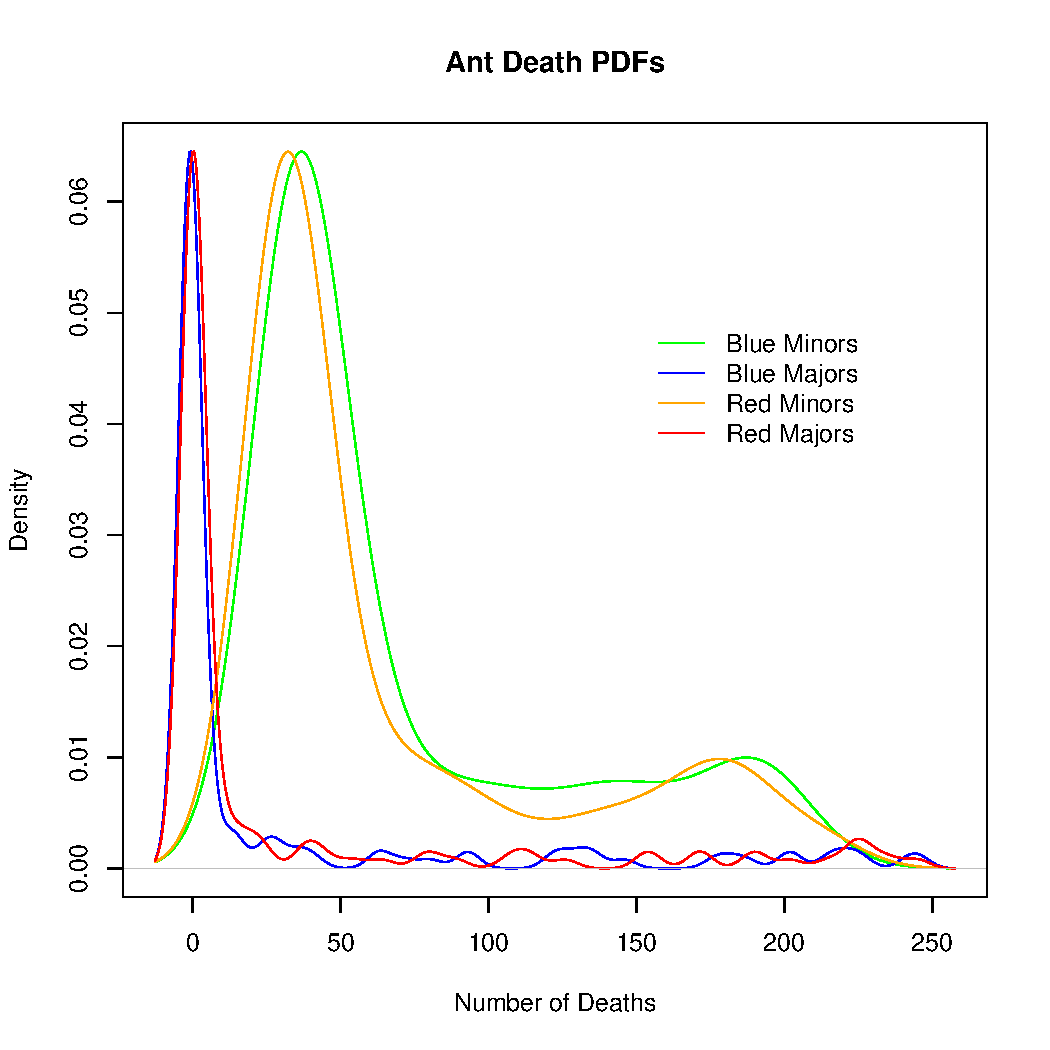
\includegraphics[scale=0.80]{partb1v1.pdf}
\caption{Probability density function for $f = 0.25, p = 0.5$}
\label{partb1fig}
\end{figure}

\begin{figure}[h!]
\centering
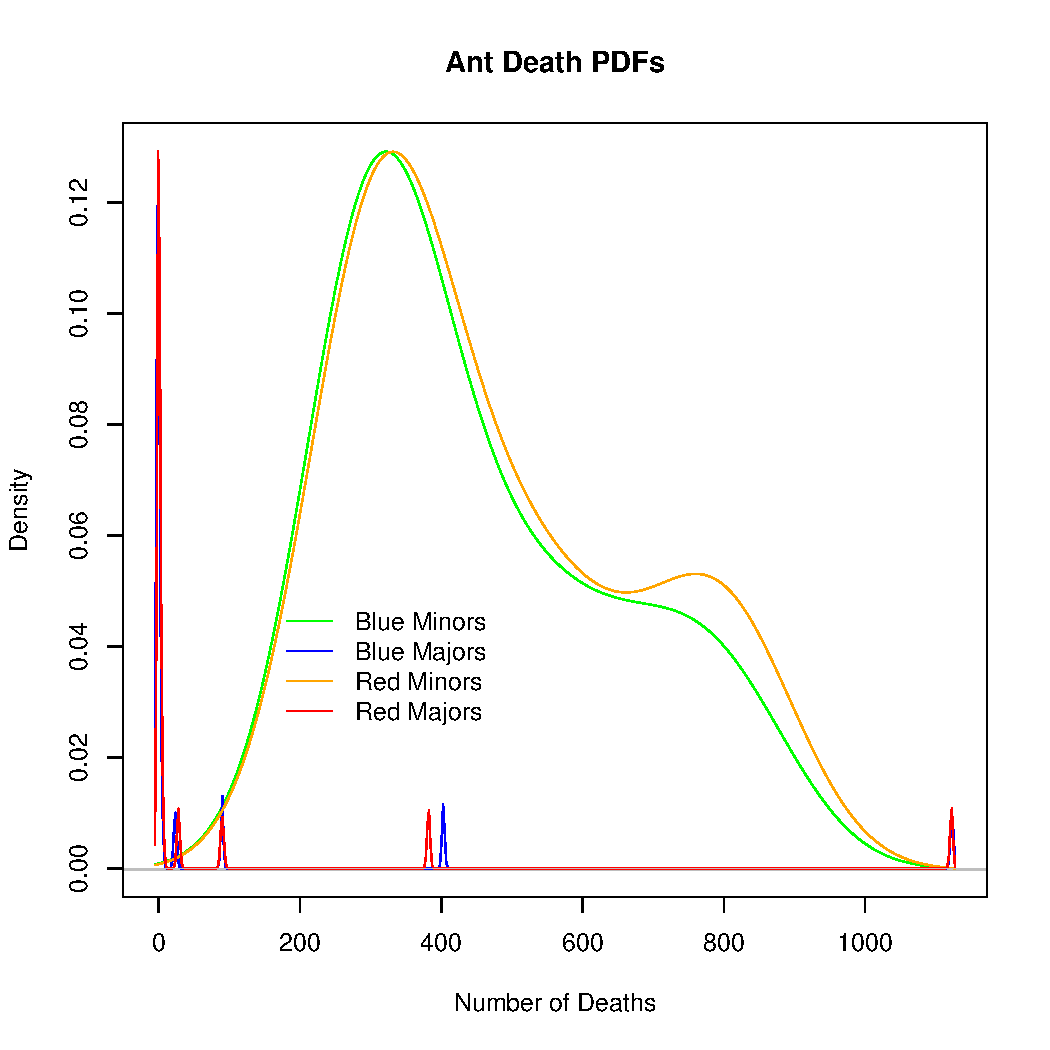
\includegraphics[scale=0.80]{partb2v1.pdf}
\caption{Probability density function for $f = 0.12, p = 0.04$}
\label{partb2fig}
\end{figure}

\begin{figure}[h!]
\centering
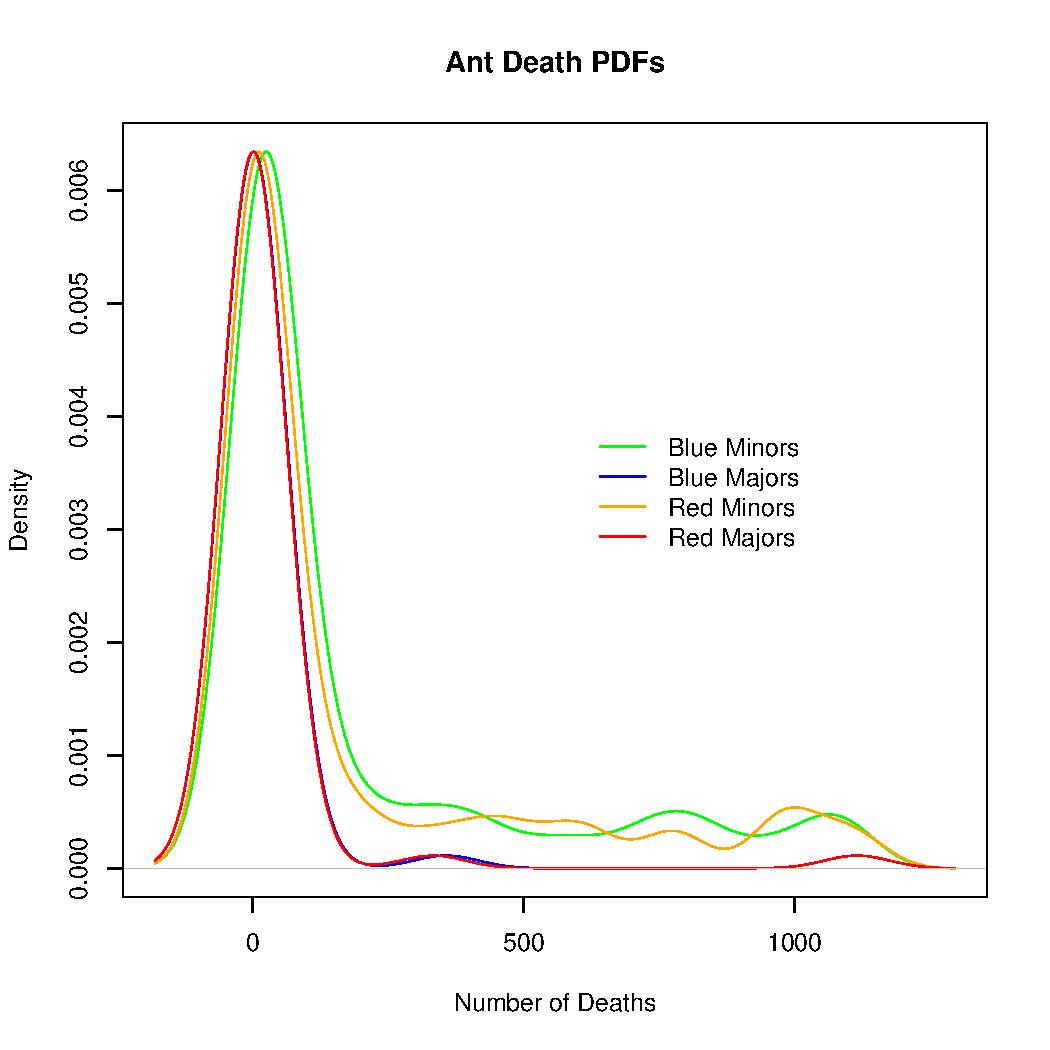
\includegraphics[scale=0.80]{partb3v1.pdf}
\caption{Probability density function for $f = 0.04, p = 0.21$}
\label{partb3fig}
\end{figure}

\item \textbf{Figure \ref{partb1fig}:}Qualitatively, setting both $p$ and $f$ to
be high allow either side to be particularly effective. The grid ends up filled 
with multiple regions for each tribe, but each region is small and their sizes
fluctuate rapidly.  The majors tend to just stick around, while the 
smaller numbers of minors means both less minor deaths (pred), and less major 
deaths (pred), with neither tribe controlling the entire grid.  The region size
also causes the long tail of major and minor ant deaths seen in the probability
density function. It is highly likely that major/minor ants end up 
sitting at the edge of an individual tribal region, so fights happen more often
in each step.  Note that screenshots of the grid for each regime are also 
included in Figs \ref{scrot1}, \ref{scrot2} and \ref{scrot3}.

\textbf{Figure \ref{partb2fig}:} This probability density function is very
different to the one in Figure \ref{partb1fig}.  Most obviously, the number 
of major deaths that occur are very small, due to the small probability that
a major ant gets born each step.  In addition, the $p$ and $f$ values allow the
minor ants to make up the bulk of ants found at the edge of one tribes region.
While the simulation runs, the minor ants appear to steadly hold the 
region edges in place.  The edges of each region mainly shift when a major ant
ends up at the edge, when it is possible for the major ant to 
break through the boundaries of the enemy tribe's region.

\textbf{Figure \ref{partb3fig}:} The probability distribution function is
different again.  In this case, there are very well defined 
regions of red and blue ants, similar to the 0.04, 0.12 case.  In this 
situation, there tend to be fewer different regions and as a result each 
red/blue region is larger.  Again, the minor ants appear to form stable edges 
to each region, while major ants born either in the empty lines or the edges of 
the coloured regions push the battlefronts into new territory.  A further 
effect of the larger territories occupied by each tribe is that the overall 
death counts for both major and minor ants are low and similar.  This is 
because most of the ants from each tribe aren't located at the edge of a tribal 
region, so they have no opportunity to get involved in battles with enemy ants.

\begin{figure}[h!]
\centering
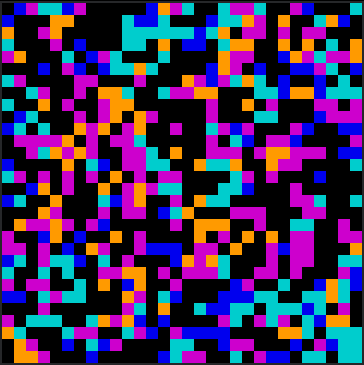
\includegraphics[scale=1.0]{partb1scrot1.png}
\caption{Grid screenshot for $f = 0.25, p = 0.5$}
\label{scrot1}
\end{figure}

\begin{figure}[h!]
\centering
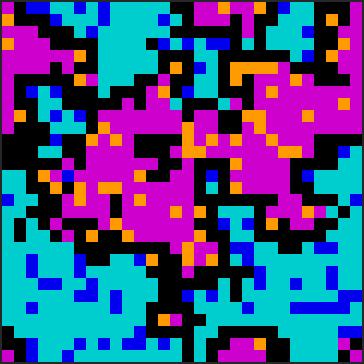
\includegraphics[scale=1.0]{partb2scrot1.png}
\caption{Grid screenshot for $f = 0.25, p = 0.5$}
\label{scrot2}
\end{figure}

\begin{figure}[h!]
\centering
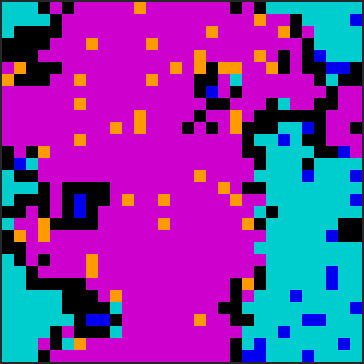
\includegraphics[scale=1.0]{partb3scrot1.png}
\caption{Grid screenshot for $f = 0.25, p = 0.5$}
\label{scrot3}
\end{figure}

\item Having different f values for the two tribes gives an immediate advantage 
to one tribe.  In the case where $p = 0.21$, ten simulations were 
run, and the number of steps taken for the board to be completely covered by a 
single tribe were logged then averaged.  The results for different values of 
$f$ are given below:

\begin{center}
\begin{tabular}{|l|l|l|l|l|}
\hline
\textbf{$f$} & \textbf{Red $p$} & \textbf{Blue $p$} & \textbf{End Colour} & \# \textbf{Steps} \\ \hline
0.21 & 0.01 & 0.04 & blue & 280 \\ \hline
0.21 & 0.025 & 0.04 & blue & 478.8 \\ \hline
0.21 & 0.035 & 0.04 & blue & 1428.7 \\ \hline
\end{tabular}
\end{center}

From the table, it is clear that as the $f$ values get closer to each other, 
the likelihood of the grid becoming completely filled by one tribe get much 
less, so it is possible to run the simulation and encounter 'interesting' 
behaviour (i.e. a grid containing two sets of battling ant tribes) for longer.

\item Adjusting the simulation to study the behaviour tribes of old and young 
ants requires some adjustments to the simulation rules.  The adjustments that 
were made are as follows:

\begin{itemize}
\item[-]Old ants are infertile, so they will never repopulate the cells of 
enemy ants they destroy.
\item[-]Young ants are fertile, so they will repopulate the cells of defeated 
ants with the same probability as when they appear on empty cells
\item[-]According to Cassil's work, "the more expendable" and ant is, "the more 
likely it is to end up in harm's way".  Thus the old ants are required to fight 
always
\item[-]The young ants will flee (if possible) if their cell is surrounded by
more enemy ants than friendly ants.  Fleeing is defined as moving into a nearby 
empty square rather than fighting.
\end{itemize}

\end{enumerate}
